\section{ÔN TẬP CHƯƠNG 2}
\subsection{TRẮC NGHIỆM NHIỀU PHƯƠNG ÁN LỰA CHỌN}
\setcounter{ex}{0}
\Opensolutionfile{ans}[ans/G10Y25B5-TN]
\begin{ex}
	Tốc độ là đại lượng đặc trưng cho
	\choice
	{\True tính chất nhanh hay chậm của chuyển động}
	{sự thay đổi hướng của chuyển động}
	{khả năng duy trì chuyển động của vật}
	{sự thay đổi vị trí của vật trong không gian}
	\loigiai{}
\end{ex}

\begin{ex}
	Đồ thị vận tốc - thời gian của chuyển động thẳng đều là một đường thẳng
	\choice
	{đi qua gốc toạ độ}
	{\True song song với trục hoành}
	{bất kì}
	{song song với trục tung}
	\loigiai{}
\end{ex}

\begin{ex}
	Chọn phát biểu đúng
	\choice
	{Vectơ độ dịch chuyển thay đổi phương liên tục khi vật chuyển động}
	{Vectơ độ dịch chuyển có độ lớn luôn bằng quãng đường đi được của chất điểm}
	{\True Khi vật chuyển động thẳng không đổi chiều, độ lớn của vectơ độ dịch chuyển bằng quãng đường đi được}
	{Vận tốc tức thời cho ta biết chiều chuyển động nên luôn có giá trị dương}
	\loigiai{}
\end{ex}

\begin{ex}
	Chỉ ra phát biểu sai.
	\choice
	{Vectơ độ dịch chuyển là một vectơ nối vị trí đầu và vị trí cuối của vật chuyển động}
	{\True Vectơ độ dịch chuyển có độ lớn luôn bằng quãng đường đi được của vật}
	{Khi vật đi từ điểm A đến điểm B, sau đó đến điểm C, rồi quay về A thì độ dịch chuyển của vật có độ lớn bằng 0}
	{Độ dịch chuyển có thể có giá trị âm, dương hoặc bằng không}
	\loigiai{}
\end{ex}

\begin{ex}
	Chuyển động nào sau đây là chuyển động thẳng nhanh dần?
	\choice
	{\True Chuyển động của ô tô khi bắt đầu chuyển động}
	{Chuyển động của xe buýt khi vào trạm}
	{Chuyển động của xe máy khi tắc đường}
	{Chuyển động của đầu kim đồng hồ}
	\loigiai{}
\end{ex}

\begin{ex}
	Một người chuyển động thẳng có độ dịch chuyển $d_1$ tại thời điểm $t_1$ và độ dịch chuyển $d_2$ tại thời điểm $t_2$. Vận tốc trung bình của vật trong khoảng thời gian từ $t_1$ đến $t_2$ là
	\choice
	{$v_{tb}=\dfrac{d_1-d_2}{t_1+t_2}$}
	{\True $v_{tb}=\dfrac{d_2-d_1}{t_2-t_1}$}
	{$v_{tb}=\dfrac{d_1+d_2}{t_2-t_1}$}
	{$v_{tb}=\dfrac{1}{2}\left(\dfrac{d_1}{t_1}+\dfrac{d_2}{t_2}\right)$}
	\loigiai{}
\end{ex}

\begin{ex}
	Tính chất nào sau đây là của vận tốc, không phải là của tốc độ của một chuyển động?
	\choice
	{Đặc trưng cho sự nhanh chậm của chuyển động}
	{Có đơn vị là $\si{\kilo\meter/\hour}$}
	{Không thể có độ lớn bằng 0}
	{\True Có phương xác định}
	\loigiai{}
\end{ex}

\begin{ex}
	Cho đồ thị độ dịch chuyển - thời gian của một vật như hình \ref{fig:0002-1}. Trong những khoảng thời gian nào thì vật chuyển động thẳng đều?
	\begin{center}
		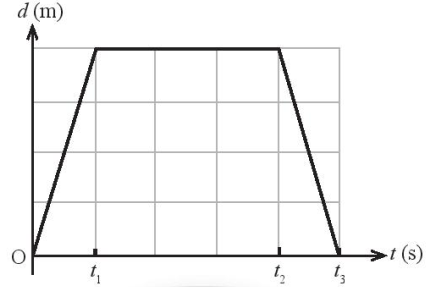
\includegraphics[scale=0.4]{figs/G10Y25B5-1}
		\captionof{figure}{}
		\label{fig:0002-1}
	\end{center}
	\choice
	{Trong khoảng thời gian từ 0 đến $t_1$ và từ $t_1$ đến $t_2$}
	{Trogn khoảng thời gian từ $t_1$ đến $t_2$}
	{Trong khoảng thời gian từ $0$ đến $t_3$}
	{\True Trong khoảng thời gian từ 0 đến $t_1$ và từ $t_2$ đến $t_3$}
	\loigiai{}
\end{ex}

\begin{ex}
	Cặp đồ thị nào dưới đây là của chuyển động thẳng đều?
	\begin{center}
		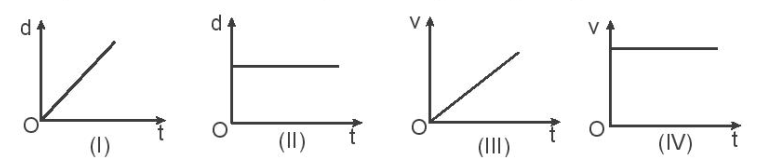
\includegraphics[scale=0.6]{figs/G10Y25B5-2}
	\end{center}
	\choice
	{I và III}
	{\True I và IV}
	{II và III}
	{II và IV}
	\loigiai{}
\end{ex}

\begin{ex}
	Hình bên là đồ thị độ dịch chuyển - thời gian của ô tô chuyển động thẳng theo một hướng xác định. Ô tô đi với tốc độ lớn nhất trong đoạn đường nào?
	\begin{center}
		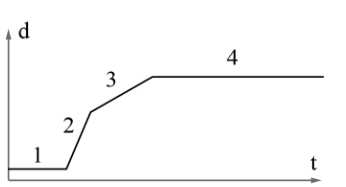
\includegraphics[scale=0.6]{figs/G10Y25B5-3}
	\end{center}
	\choice
	{1}
	{\True 2}
	{3}
	{4}
	\loigiai{}
\end{ex}

\begin{ex}
	Tàu Thống Nhất TN1 đi từ ga Huế vào ga Sài Gòn mất $\SI{20}{\hour}$. Biết tốc độ trung bình của tàu là $\SI{15}{\meter/\second}$. Hỏi chiều dài của đường ray từ Huế vào Sài Gòn?
	\choice
	{$\SI{3000}{\kilo\meter}$}
	{\True $\SI{1080}{\kilo\meter}$}
	{$\SI{1000}{\kilo\meter}$}
	{$\SI{1333}{\kilo\meter}$}
	\loigiai{
		Chiều dài của đường ray từ Huế vào Sài Gòn:
		$$s=vt=\SI{1080}{\kilo\meter}$$
	}
\end{ex}

\begin{ex}
	Trong trận đấu giữa Đức và Áo ở EURO 2008, tiền vệ Michael Ballack của đội tuyển Đức sút phạt cách khung thành của đội Áo $\SI{30}{\meter}$. Các chuyên gia tính được tốc độ trung bình của quả phạt đó lên tới $\SI{108}{\kilo\meter/\hour}$. Hỏi thời gian bay của quả bóng là bao nhiêu?
	\choice
	{\True $\SI{1}{\second}$}
	{$\SI{36}{\second}$}
	{$\SI{1.5}{\second}$}
	{$\SI{3.6}{\second}$}
	\loigiai{
		Thời gian bay của quả bóng:
		$$t=\dfrac{s}{v} = \SI{1}{\second}$$
	}
\end{ex}

\begin{ex}
	Hưng đạp xe lên dốc dài $\SI{100}{\meter}$ với vận tốc $\SI{2}{\meter/\second}$, sau đó xuống dốc dài $\SI{140}{\meter}$ hết $\SI{30}{\second}$. Hỏi tốc độ trung bình của Hưng trên cả hai đoạn đường?
	\choice
	{$\SI{50}{\meter/\second}$}
	{$\SI{8}{\meter/\second}$}
	{$\SI{4.67}{\meter/\second}$}
	{\True $\SI{3}{\meter/\second}$}
	\loigiai{
		Thời gian trên đoạn đường thứ nhất:
		$$t_1=\dfrac{s_1}{v_1} = \SI{50}{\second}$$
		Tốc độ trung bình trên cả hai đoạn đường:
		$$v=\dfrac{s_1+s_2}{t_1+t_2} = \SI{3}{\meter/\second}$$
	}
\end{ex}

\begin{ex}
	Đồ thị toạ độ - thời gian của hai xe 1 và 2 được biểu diễn như hình \ref{fig:0002-2}. Hai xe gặp nhau tại vị trí cách vị trí xuất phát của 2 xe một khoảng
	\begin{center}
		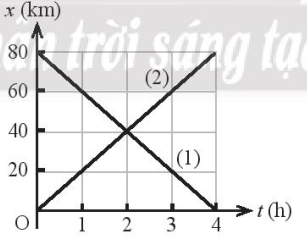
\includegraphics[scale=0.5]{figs/G10Y25B5-4}
		\captionof{figure}{}
		\label{fig:0002-2}
	\end{center}
	\choice
	{\True $\SI{40}{\kilo\meter}$}
	{$\SI{30}{\kilo\meter}$}
	{$\SI{35}{\kilo\meter}$}
	{$\SI{70}{\kilo\meter}$}
	\loigiai{}
\end{ex}

\begin{ex}
	Phương trình chuyển động và độ lớn vận tốc của hai chuyển động có đồ thị như hình bên là
	\begin{center}
		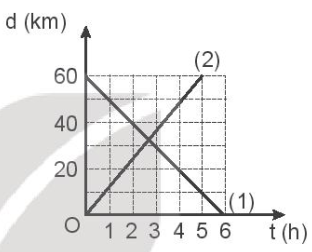
\includegraphics[scale=0.5]{figs/G10Y25B5-5}
	\end{center}
	\choice
	{\True $d_1=\xsi{60-10t}{\kilo\meter}; v_1=\SI{10}{\kilo\meter/\hour}$\\$d_2=\xsi{12t}{\kilo\meter}; v_2=\SI{12}{\kilo\meter/\hour}$}
	{$d_1=\xsi{60+10t}{\kilo\meter}; v_1=\SI{10}{\kilo\meter/\hour}$\\$d_2=\xsi{-10t}{\kilo\meter}; v_2=\SI{10}{\kilo\meter/\hour}$}
	{$d_1=\xsi{60-20t}{\kilo\meter}; v_1=\SI{20}{\kilo\meter/\hour}$\\$d_2=\xsi{12t}{\kilo\meter}; v_2=\SI{12}{\kilo\meter/\hour}$}
	{$d_1=\xsi{-10t}{\kilo\meter}; v_1=\SI{10}{\kilo\meter/\hour}$\\$d_2=\xsi{12t}{\kilo\meter}; v_2=\SI{12}{\kilo\meter/\hour}$}
	\loigiai{
		Độ lớn vận tốc của mỗi xe
		\begin{align*}
			\begin{cases}
				\left|v_1\right|=\dfrac{\left|0-60\right|}{6}=\SI{10}{\kilo\meter/\hour}\\
				\left|v_2\right|=\dfrac{\left|60-0\right|}{5}=\SI{12}{\kilo\meter/\hour}
			\end{cases}
		\end{align*}
		Phương trình chuyển động của hai xe:
		\begin{align*}
			\begin{cases}
				d_1=\xsi{60-10t}{\kilo\meter}\\
				d_2=\xsi{12t}{\kilo\meter}
			\end{cases}
		\end{align*}
	}
\end{ex}

\begin{ex}
	Hãy thiết lập phương trình chuyển động của một ô tô chuyển động thẳng đều biết. Ô tô chuyển động theo chiều dương với vận tốc $\SI{10}{\meter/\second}$ và ở thời điểm $\SI{3}{\second}$ thì vật có tọa độ $\SI{60}{\meter}$.
	\choice
	{\True $\xsi{30+10t}{\meter}$}
	{$\xsi{20+10t}{\meter}$}
	{$\xsi{10+20t}{\meter}$}
	{$\xsi{40+10t}{\meter}$}
	\loigiai{
		Phương trình chuyển động của ô tô:
		$$x=x_0+\SI{10}{t}$$
		Khi $t=\SI{3}{\second}$ thì vật có toạ độ $x=\SI{60}{\meter}\Rightarrow x_0=\SI{30}{\meter}.$
	}
\end{ex}

\begin{ex}
	Lúc 7 giờ sáng, tại A xe thứ nhất chuyển động thẳng đều với tốc độ $\SI{12}{\kilo\meter/\hour}$ để về B. Một giờ sau, tại B xe thứ hai cũng chuyển động thẳng đều với tốc độ $\SI{48}{\kilo\meter/\hour}$ theo chiều ngược lại để về A. Cho đoạn thẳng $AB=\SI{72}{\kilo\meter}$. Khoảng cách giữa hai xe lúc 10 giờ là
	\choice
	{$\SI{12}{\kilo\meter}$}
	{\True $\SI{60}{\kilo\meter}$}
	{$\SI{36}{\kilo\meter}$}
	{$\SI{24}{\kilo\meter}$}
	\loigiai{
		Chọn gốc toạ độ tại A, chiều dương hướng từ A đến B. Chọn gốc thời gian lúc $\SI{7}{\hour}$.
		Phương trình chuyển động của mỗi xe:
		\begin{align*}
			\begin{cases}
				x_1=\xsi{12t}{\kilo\meter}\\
				x_2=\xsi{72-48(t-1)}{\kilo\meter}
			\end{cases}
		\end{align*}
		Khoảng cách hai xe lúc $\SI{10}{\hour}$, tương ứng $t=\SI{3}{\hour}$:
		$$\Delta x=\left|x_1-x_2\right|=\SI{60}{\kilo\meter}$$
	}
\end{ex}

\begin{ex}
	Một chiếc máy bay đang bay từ Thành phố Hồ Chí Minh đến Thủ đô Hà Nội với tốc độ $\SI{525}{\kilo\meter/\hour}$. Trong hôm đó, gió thổi về hướng Nam với tốc độ $\SI{36}{\kilo\meter/\hour}$. Xem như máy bay chuyển động thẳng đều theo hướng Bắc và quãng đường bay từ Thành phố Hồ Chí Minh đến Thủ đô Hà Nội là $\SI{1160}{\kilo\meter}$. Hãy xác định thời gian bay của máy bay trên quãng đường đó.
	\choice
	{$\SI{3,27}{\hour}$}
	{$\SI{7,32}{\hour}$}
	{$\SI{1,37}{\hour}$}
	{\True $\SI{2,37}{\hour}$}
	\loigiai{
		Gọi:
		$\vec v_{1,2}$ là vận tốc của máy bay so với gió.
		$\vec v_{2,3}$ là vận tốc của gió so với mặt đất.
		$\vec v_{1,3}$ là vận tốc của máy bay so với mặt đất.
		Ta có:
		$$\vec v_{1,3} = \vec v_{1,2} + \vec v_{2,3}.$$
		Tốc độ của máy bay so với gió là $v_{1,2}= \SI{525}{\kilo\meter/\hour}$; tốc độ của gió so với mặt đất là $ v_{2,3}= \SI{36}{\kilo\meter/\hour}$.
		Chọn chiều dương là chiều chuyển động của máy bay (hướng bắc).
		Do gió chuyển động theo hướng nam nên: $v_{2,3} <0$.
		Vận tốc của máy bay:
		$$v_{1,3} = v_{1,2} - v_{2,3} = \SI{489}{\kilo\meter/\hour}.$$
		Thời gian bay của máy bay trên quãng đường $\SI{1160}{\kilo\meter}$ là:
		$$ t =\dfrac{S}{v} \approx \SI{2,37}{\hour}.$$
	}
\end{ex}

\begin{ex}
	Một chiếc ô tô chạy từ điểm A đến điểm B. Nửa đoạn đường đầu ô tô đi với tốc độ $v_1=\SI{40}{\kilo\meter/\hour}$. Trong quãng thời gian còn lại thì một nửa quãng thời gian đầu ô tô đi với tốc độ $v_2=\SI{50}{\kilo\meter/\hour}$, một nửa quãng thời gian cuối ô tô đi với tốc độ $v_3=\SI{60}{\kilo\meter/\hour}$. Tính tốc độ trung bình của ô tô trên cả đoạn đường AB.
	\choice
	{\True $\SI{46.3}{\kilo\meter/\hour}$}
	{$\SI{55.7}{\kilo\meter/\hour}$}
	{$\SI{57.4}{\kilo\meter/\hour}$}
	{$\SI{58.5}{\kilo\meter/\hour}$}
	\loigiai{}
\end{ex}

\begin{ex}
	Một chiếc ô tô chạy từ điểm A đến điểm B. Nửa quãng thời gian đầu ô tô đi với tốc độ $v_1=\SI{40}{\kilo\meter/\hour}$. Trong quãng thời gian còn lại thì một nửa quãng thời gian đầu ô tô đi với tốc độ $v_2=\SI{50}{\kilo\meter/\hour}$, một nửa quãng thời gian cuối ô tô đi với tốc độ $v_3=\SI{60}{\kilo\meter/\hour}$. Tính tốc độ trung bình của ô tô trên cả đoạn đường AB.
	\choice
	{$\SI{45.5}{\kilo\meter/\hour}$}
	{\True $\SI{47.5}{\kilo\meter/\hour}$}
	{$\SI{57.5}{\kilo\meter/\hour}$}
	{$\SI{55.5}{\kilo\meter/\hour}$}
	\loigiai{}
\end{ex}
\Closesolutionfile{ans}
\subsection{TRẮC NGHIỆM ĐÚNG SAI}
\setcounter{ex}{0}
\Opensolutionfile{ans}[ans/G10Y25B5-TF]


\Closesolutionfile{ans}
\subsection{TRẢ LỜI NGẮN}
\setcounter{ex}{0}
\Opensolutionfile{ans}[ans/G10Y25B5-SA]


\Closesolutionfile{ans}
\subsection{TỰ LUẬN}
\setcounter{ex}{0}
\Opensolutionfile{ans}[ans/G10Y25B5-TL]

\begin{ex}
	Hình \ref{fig:0002-3} mô tả đồ thị toạ độ - thời gian của hai xe, hãy nêu đặc điểm chuyển động của mỗi xe.
	\begin{center}
		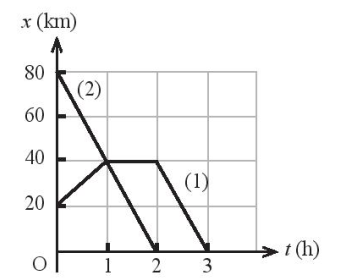
\includegraphics[scale=0.5]{figs/G10Y25B5-6}
		\captionof{figure}{Đồ thị toạ độ - thời gian của hai xe}
		\label{fig:0002-3}
	\end{center}
	\loigiai{
		\begin{itemize}
			\item \text{Chuyển động của xe 1:}
			\begin{itemize}
				\item \text{Trong khoảng thời gian từ } $\SI{0}{\hour}$ \text{đến } $\SI{1}{\hour}$, \text{xe chuyển động đều theo chiều dương với tốc độ } $\SI{20}{\kilo\meter/\hour}$.
				\item \text{Trong khoảng thời gian từ } $\SI{1}{\hour}$ \text{đến } $\SI{2}{\hour}$, \text{xe đứng yên}.
				\item \text{Trong khoảng thời gian từ } $\SI{2}{\hour}$ \text{đến } $\SI{3}{\hour}$, \text{xe chuyển động đều theo chiều âm với tốc độ } $\SI{40}{\kilo\meter/\hour}$.
			\end{itemize}
			\item \text{Chuyển động của xe 2: Trong khoảng thời gian từ } $\SI{0}{\hour}$ \text{đến } $\SI{2}{\hour}$, \text{xe chuyển động đều theo chiều âm với tốc độ } $\SI{40}{\kilo\meter/\hour}$
		\end{itemize}
	}
\end{ex}

\begin{ex}
	Hình \ref{fig:0002-4} mô tả đồ thị độ dịch chuyển - thời gian của một chiếc xe ô tô chạy trên đường thẳng. Tính vận tốc trung bình của xe.
	\begin{center}
		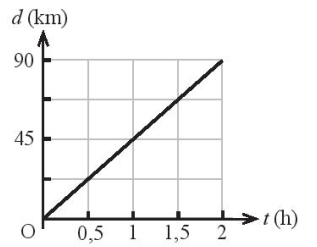
\includegraphics[scale=0.6]{figs/G10Y25B5-7}
		\captionof{figure}{Đồ thị độ dịch chuyển - thời gian của xe}
		\label{fig:0002-4}
	\end{center}
	\loigiai{
		\text{Vận tốc trung bình của xe}
		$$v=\dfrac{\Delta d}{\Delta t}=\SI{45}{\kilo\meter/\hour}.$$
	}
\end{ex}

\begin{ex}
	Trong Hình \ref{fig:0002-5} có hai băng giấy ghi lại vị trí của vật chuyển động sau những khoảng thời gian bằng nhau. Hãy mô tả chuyển động của hai vật trong hai trường hợp này.
	\begin{center}
		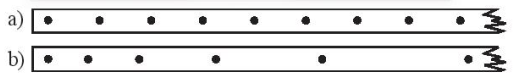
\includegraphics[scale=0.5]{figs/G10Y25B5-8}
		\captionof{figure}{Băng giấy ghi lại vị trí của vật chuyển động}
		\label{fig:0002-5}
	\end{center}
	\loigiai{
		\begin{enumerate}[label=\alph*)]
			\item \text{Vật chuyển động thẳng đều}.
			\item \text{Vật chuyển động thẳng nhanh dần}.
		\end{enumerate}
	}
\end{ex}

\begin{ex}
	Trái Đất quay quanh một vòng quanh Mặt Trời trong khoảng thời gian gần 1 năm. Tính tốc độ trung bình và vận tốc trung bình của Trái Đất khi nó hoàn thành một vòng quay quanh Mặt Trời. Xem chuyển động này gần đúng là chuyển động tròn và khoảng cách từ Trái Đất đến Mặt Trời khoảng $\SI{1.5E11}{\meter}$.
	
	\loigiai{
		\text{Xem Trái Đất chuyển động tròn xung quanh Mặt Trời, như vậy quãng đường Trái Đất di chuyển trong 1 năm bằng chu vi đường tròn bán kính } $R=\SI{1.5E11}{\meter}$:
		$$s=2\pi R$$
		\text{Sau 1 năm, Trái Đất đi hết chiều dài quỹ đạo và trở về vị trí ban đầu, do đó:}
		$$d=0$$
		\begin{itemize}
			\item \text{Tốc độ trung bình } $$v_{tb}=\dfrac{s}{t}=\dfrac{2\pi\cdot\left(\SI{1.5E11}{\meter}\right)}{}\approx\SI{11E4}{\kilo\meter/\hour}$$
			\item \text{Vận tốc trung bình } $$v=\dfrac{d}{t}=0.$$
		\end{itemize}
	}
\end{ex}

\begin{ex}
	Một tàu ngầm sử dụng hệ thống phát sóng âm để đo độ sâu của biển. Hệ thống phát ra sóng âm và đo thời gian quay trở lại của sóng âm sau khi chúng bị phản xạ tại đáy biển. Tại một vị trí trên mặt biển, thời gian mà hệ thống ghi nhận được là $\SI{0.13}{\second}$ kể từ khi sóng âm được truyền đi. Tính độ sâu mực nước biển. Biết tốc độ truyền âm trong nước khoảng $\SI{1500}{\meter/\second}$.
	
	\loigiai{
		\text{Độ sâu của mực nước biển:}
		$$h=v\cdot\dfrac{t}{2}=\SI{97.5}{\meter}.$$
	}
\end{ex}

\begin{ex}
	Một người đi xe máy từ nhà đến bến xe buýt cách nhà $\SI{6}{\kilo\meter}$ về phía đông. Đến bến xe, người đó lên xe buýt đi tiếp $\SI{20}{\kilo\meter}$ về phía bắc.
	\begin{enumerate}[label=\alph*)]
		\item Tính quãng đường được trong cả chuyến đi.
		\item Xác định độ dịch chuyển tổng hợp của người đó.
	\end{enumerate}
	\loigiai{
		\begin{enumerate}[label=\alph*)]
			\item \text{Quãng đường đi được:}
			$$s=6+20=\SI{26}{\kilo\meter}$$
			\item \text{Độ dịch chuyển:}
			$$d=\sqrt{6^2+20^2}\approx\SI{20.88}{\kilo\meter}.$$
		\end{enumerate}
	}
\end{ex}


\begin{ex}
	Em của An chơi trò chơi tìm kho báu ở ngoài vườn với các bạn của mình. Em của An giấu kho báu của mình là một chiếc vòng nhựa vào trong một chiếc giày rồi viết mật thư tìm kho báu như sau: bắt đầu từ gốc cây ổi, đi 10 bước về phía bắc, sau đó đi 4 bước về phía tây, 15 bước về phía nam, 5 bước về phía đông và 5 bước về phía bắc là tới chỗ giấu kho báu.
	\begin{enumerate}[label=\alph*)]
		\item Hãy tính quãng đường phải đi (theo bước) để tìm kho báu.
		\item Kho báu được giấu ở vị trí nào?
		\item Tính độ dịch chuyển (theo bước) để tìm ra kho báu.
	\end{enumerate}
	
	\loigiai{
		\begin{center}
			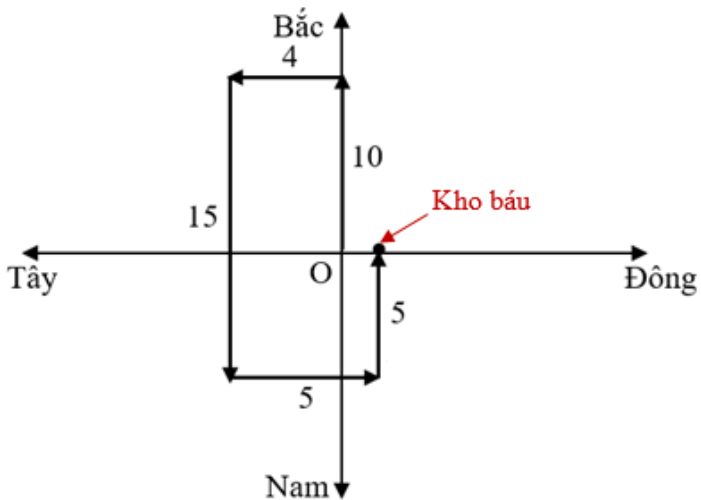
\includegraphics[scale=0.4]{figs/G10Y25B5-9}
		\end{center}
		\begin{enumerate}[label=\alph*)]
			\item $s=4+15+5+5=\text{39 bước}$.
			\item \text{Cách cây ổi 1 bước theo hướng đông}.
			\item $d=\text{1 bước (hướng đông)}$.
		\end{enumerate}
	}
\end{ex}


\begin{ex}
	Một ô tô đang chạy với vận tốc $v$ theo phương nằm ngang thì người ngồi trong xe trông thấy giọt mưa rơi tạo thành những vạch làm với phương thẳng đứng một góc $\SI{45}{\degree}$. Biết tốc độ của các giọt mưa so với mặt đất là $\SI{5}{\meter/\second}$. Xác định vận tốc của ô tô.
	
	\loigiai{
		\text{Gọi:}
		\begin{itemize}
			\item (1) \text{là giọt mưa};
			\item (2) \text{là xe};
			\item (3) \text{là mặt đường}.
		\end{itemize}
		\text{Vận tốc của giọt mưa so với xe:}
		$$\vec v_{12}=\vec v_{13}-\vec v_{23}$$
		\begin{center}
			\begin{tikzpicture}
				\coordinate (O) at (0,0);
				\coordinate (B) at (4,0);
				\coordinate (C) at (-4,0);
				\coordinate (D) at (0,4);
				\tkzMarkRightAngle[size=0.3,color=cyan](D,O,C);
				\foreach \i in {O}{
					\filldraw[black] (\i) circle (0.05);
				}
				\draw[-stealth,thick, red] (D) -- (O);
				\draw[-stealth,thick, blue] (O) -- (B);
				\draw[-stealth,thick, blue] (O) -- (C);
				\draw[-stealth,thick] (D) -- (C);
				\node[label={[red,below right]90:$\vec v_{13}$}] at (0,2){};	
				\node[label={[blue,below]90:$\vec v_{23}$}] at (2,0){};	
				\node[label={[blue,below]90:$-\vec v_{23}$}] at (-2,0){};	
				\node[label={[black,left]90:$\vec v_{12}$}] at (-2,2){};
				\tkzMarkAngle[size=0.6,color=black](C,D,O);
				\tkzLabelAngle[color=black,pos=1.2](C,D,O){$\SI{45}{\degree}$}
				
			\end{tikzpicture}
		\end{center}
		\text{Độ lớn vận tốc của ô tô (so với mặt đường):}
		$$v_{23}=v_{13} \tan\SI{45}{\degree}=\SI{5}{\meter/\second}$$
		\text{Vận tốc của ô tô có độ lớn } $\SI{5}{\meter/\second}$ \text{và có phương làm với phương chuyển động của giọt mưa để lại trên mặt kính một góc } $\SI{135}{\degree}$.
	}
\end{ex}

\begin{ex}
	Một ca nô chạy ngang qua một dòng sông, xuất phát từ A, hướng mũi về B. Sau $\SI{100}{\second}$, ca nô cập bờ bên kia ở điểm C cách B $\SI{200}{\meter}$. Nếu người lái hướng mũi ca nô theo hướng AD và vẫn giữ tốc độ máy như cũ thì ca nô sẽ cập bờ bên kia tại đúng điểm B. Tìm
	\begin{center}
		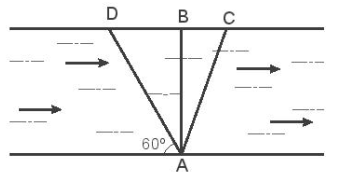
\includegraphics[scale=0.35]{figs/G10Y25B5-10}
	\end{center}
	\begin{enumerate}[label=\alph*)]
		\item Vận tốc của dòng nước so với bờ sông.
		\item Vận tốc của ca nô so với dòng nước.
		\item Chiều rộng của sông.
	\end{enumerate}
	\loigiai{
		\begin{enumerate}[label=\alph*)]
			\item \text{Gọi:}
			\begin{itemize}
				\item $\vec v_{12}$ \text{là vận tốc của ca nô so với dòng nước};
				\item $\vec v_{23}$ \text{là vận tốc của dòng nước so với bờ sông};
				\item $\vec v_{13}$ \text{là vận tốc của ca nô so với bờ sông}.
			\end{itemize}
			\begin{center}
				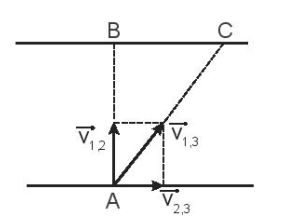
\includegraphics[scale=0.3]{figs/G10Y25B5-11}
			\end{center}
			\text{Khi mũi ca nô hướng về B thì}
			$$\vec v_{13}=\vec v_{12}+\vec v_{23}$$
			\text{với } $v_{12}=\dfrac{AB}{t}$ \text{và } $v_{23}=\dfrac{BC}{t}=\dfrac{\SI{200}{\meter}}{\SI{100}{\second}}=\SI{2}{\meter/\second}$.\\
			\item \text{Khi mũi ca nô hướng về D thì }
			\begin{center}
				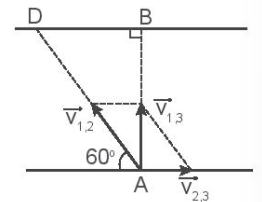
\includegraphics[scale=0.5]{figs/G10Y25B5-13}
			\end{center}
			$$\overrightarrow v'_{13}=\overrightarrow v'_{12}+\overrightarrow v'_{23}$$
			\text{với } $v'_{12}=v_{12}$ \text{và } $v'_{23}=v_{23}=\SI{2}{\meter/\second}$.\\
			\text{Ta có:}
			$$v'_{12}=\dfrac{v'_{12}}{\sin\SI{30}{\degree}}=\SI{4}{\meter/\second}$$
			\item $AB=v_{12}\cdot t=\SI{400}{\meter}$.
		\end{enumerate}
	}
\end{ex}

\begin{ex}
	Một tàu ngầm đang lặn xuống theo phương thẳng đứng với vận tốc không đổi $v$. Máy sonar định vị của tàu phát tín hiệu siêu âm theo phương thẳng đứng xuống đáy biển. Biết thời gian tín hiệu đi xuống đáy biển là $t_1$, thời gian tín hiệu phản hồi từ đáy biển tới tàu là $t_2$, vận tốc của siêu âm trong nước biển là $u$ và đáy biển nằm ngang. Tính vận tốc lặn $v$ của tàu theo $u$, $t_1$ và $t_2$.
	
	\loigiai{
		\begin{center}
			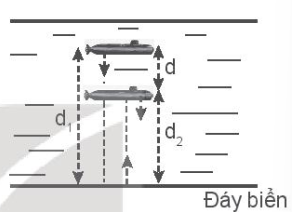
\includegraphics[scale=0.5]{figs/G10Y25B5-12}
		\end{center}
		\text{Trong thời gian } $\left(t_1+t_2\right)$, \text{con tàu đã lặn sâu được một đoạn } $d=v\left(t_1+t_2\right)\Rightarrow v=\dfrac{d}{t_1+t_2}$.\\
		\text{Trong thời gian } $t_1$, \text{tín hiệu phát truyền được một đoạn } $d_2=ut_2$\\
		\text{Vì } $d=d_1-d_2=u\left(t_1-t_2\right)$\\
		$\Rightarrow v=u\cdot\left(\dfrac{t_1-t_2}{t_1+t_2}\right)$.
	}
\end{ex}
\Closesolutionfile{ans}